%%%%%%%%%%%%%%%%%%%%%%%%%%%%%%%%%%%%%%%%%%%%%%%%%%%%%%%%%%%%
%%% LIVECOMS ARTICLE TEMPLATE FOR BEST PRACTICES GUIDE
%%% ADAPTED FROM ELIFE ARTICLE TEMPLATE (8/10/2017)
%%%%%%%%%%%%%%%%%%%%%%%%%%%%%%%%%%%%%%%%%%%%%%%%%%%%%%%%%%%%
%%% PREAMBLE
\documentclass[9pt,bestpractices,pubversion]{livecoms}
% Use the 'onehalfspacing' option for 1.5 line spacing
% Use the 'doublespacing' option for 2.0 line spacing
% Use the 'lineno' option for adding line numbers.
% The 'bestpractices' option for indicates that this is a best practices guide.
% Omit the bestpractices option to remove the marking as a LiveCoMS paper.
% Please note that these options may affect formatting.

\usepackage{lipsum} % Required to insert dummy text
\usepackage[version=4]{mhchem}
\usepackage{siunitx}
\usepackage{url}
\DeclareSIUnit\Molar{M}
\usepackage[italic]{mathastext}
\graphicspath{{figures/}}

%%%%%%%%%%%%%%%%%%%%%%%%%%%%%%%%%%%%%%%%%%%%%%%%%%%%%%%%%%%%
%%% IMPORTANT USER CONFIGURATION
%%%%%%%%%%%%%%%%%%%%%%%%%%%%%%%%%%%%%%%%%%%%%%%%%%%%%%%%%%%%
\usepackage[colorinlistoftodos]{todonotes}
\usepackage[most]{tcolorbox}
\usepackage{enumitem,amssymb}
\usepackage{textgreek}
\usepackage{changepage}

%%%%%%%%%%%%%%%%%%%%%%%%%%%%%%%%%%%%%%%%%%%%%%%%%%%%%%%%%%%%
%%% Added to allow customisation of table of contents
%%%%%%%%%%%%%%%%%%%%%%%%%%%%%%%%%%%%%%%%%%%%%%%%%%%%%%%%%%%%
\usepackage{tocloft}
\usepackage{xcolor}
\usepackage{todonotes}

% Define custom commands for colored TOC entries
\newcommand{\tocgreen}[1]{\textcolor{green}{#1}}
\newcommand{\tocorange}[1]{\textcolor{orange}{#1}}
\newcommand{\tocred}[1]{\textcolor{red}{#1}}

% Define custom commands for TOC entries with comments
\makeatletter
\newcommand{\tocsectioncomment}[1]{%
  \addtocontents{toc}{%
    {\leftskip \cftsecindent\relax
     \advance\leftskip \cftsecnumwidth\relax
     \rightskip \@tocrmarg\relax
     \textit{#1}\protect\par}}%
  \textit{#1}\par}

% Command for subsection comments in TOC
\newcommand{\tocsubsectioncomment}[1]{%
  \addtocontents{toc}{%
    {\leftskip \cftsubsecindent\relax
     \advance\leftskip \cftsubsecnumwidth\relax
     \rightskip \@tocrmarg\relax
     \textit{#1}\protect\par}}%
  \textit{#1}\par}

% Command for subsubsection comments in TOC
\newcommand{\tocsubsubsectioncomment}[1]{%
  \addtocontents{toc}{%
    {\leftskip \cftsubsecindent\relax
     \advance\leftskip \cftsubsubsecnumwidth\relax
     \rightskip \@tocrmarg\relax
     \textit{#1}\protect\par}}%
  \textit{#1}\par}

\makeatother

%%%%%%%%%%%%%%%%%%%%%%%%%%%%%%%%%%%%%%%%%%%%%%%%%%%%%%%%%%%%

\newcommand{\versionnumber}{0.1} % you should update the minor version number in preprints and major version number of submissions.
\newcommand{\githubrepository}{\url{https://github.com/alchemistry/alchemical-best-practices}} %this should be the main github repository for this article
\newcommand{\expect}[1]{\left\langle{#1}\right\rangle}
%%%%%%%%%%%%%%%%%%%%%%%%%%%%%%%%%%%%%%%%%%%%%%%%%%%%%%%%%%%%
%%% ARTICLE SETUP
%%%%%%%%%%%%%%%%%%%%%%%%%%%%%%%%%%%%%%%%%%%%%%%%%%%%%%%%%%%%
\title{Best Practices for Multiple Alchemical Free Energy Calculations [Article v\versionnumber]}
\author[1*]{Antonia S. J. S. Mey}
\author[2]{Bryce K. Allen}
\author[3]{Hannah E. Bruce Macdonald}
\author[3*]{John D. Chodera}
\author[9]{David F. Hahn}
\author[1,10]{Maximilian Kuhn}
\author[1]{Julien Michel}
\author[4*]{David L. Mobley}
\author[5]{Levi N. Naden}
\author[6]{Samarjeet Prasad}
\author[2,7]{Andrea Rizzi}
\author[1]{Jenke Scheen}
\author[8*]{Michael R. Shirts}
\author[9]{Gary Tresadern}
\author[2]{Huafeng Xu}
%
\affil[1]{EaStCHEM School of Chemistry, David Brewster Road, Joseph Black Building, The King's Buildings, Edinburgh, EH9 3FJ, UK}
\affil[2]{Silicon Therapeutics, Boston, MA, USA}
\affil[3]{Computational and Systems Biology Program, Sloan Kettering Institute, Memorial Sloan Kettering Cancer Center, New York NY, USA}
\affil[4]{Departments of Pharmaceutical Sciences and Chemistry, University of California, Irvine, Irvine, USA}
\affil[5]{Molecular Sciences Software Institute, Blacksburg VA, USA}
\affil[6]{National Institutes of Health, Bethesda, MD, USA}
\affil[7]{Tri-Institutional Training Program in Computational Biology and Medicine, New York, NY, USA}
\affil[8]{University of Colorado Boulder, Boulder, CO, USA}
\affil[9]{Computational Chemistry, Janssen Research \& Development, Turnhoutseweg 30, Beerse B-2340, Belgium}
\affil[10]{Cresset, Cambridgeshire, UK}

%
\corr{antonia.mey@ed.ac.uk}{ASJSM}
\corr{john.chodera@choderalab.org}{JDC}
\corr{dmobley@mobleylab.org}{DLM}
\corr{michael.shirts@colorado.edu}{MRS}

\orcid{Antonia S. J. S. Mey}{0000-0001-7512-5252}
\orcid{Bryce Allen}{0000-0002-0804-8127}
\orcid{Hannah E. Bruce Macdonald}{0000-0002-5562-6866}
\orcid{John D. Chodera}{0000-0003-0542-119X}
\orcid{Maximilian Kuhn}{0000-0002-2811-3934}
\orcid{Julien Michel}{0000-0003-0360-1760}
\orcid{David L. Mobley}{0000-0002-1083-5533}
\orcid{Levi N. Naden}{0000-0002-3692-5027}
\orcid{Samarjeet Prasad}{0000-0001-8320-6482}
\orcid{Andrea Rizzi}{0000-0001-7693-2013}
\orcid{Jenke Scheen}{0000-0001-9781-0445}
\orcid{Michael R. Shirts}{0000-0003-3249-1097}
\orcid{Gary Tresadern}{0000-0002-4801-1644}
\orcid{Huafeng Xu}{0000-0001-5447-0452}
\orcid{David F. Hahn}{0000-0003-2830-6880}

\blurb{This LiveCoMS document is maintained online on GitHub at \githubrepository; to provide feedback, suggestions, or help improve it, please visit the GitHub repository and participate via the issue tracker.}

%%%%%%%%%%%%%%%%%%%%%%%%%%%%%%%%%%%%%%%%%%%%%%%%%%%%%%%%%%%%
%%% PUBLICATION INFORMATION
%%% Fill out these parameters when available
%%% These are used when the "pubversion" option is invoked
%%%%%%%%%%%%%%%%%%%%%%%%%%%%%%%%%%%%%%%%%%%%%%%%%%%%%%%%%%%%
\pubDOI{10.33011/livecoms.2.1.18378}
\pubvolume{2}
\pubyear{2020}
\articlenum{18378}
\datereceived{5 August 2020}
\dateaccepted{25 November 2020}

%%%%%%%%%%%%%%%%%%%%%%%%%%%%%%%%%%%%%%%%%%%%%%%%%%%%%%%%%%%%
%%% ARTICLE START
%%%%%%%%%%%%%%%%%%%%%%%%%%%%%%%%%%%%%%%%%%%%%%%%%%%%%%%%%%%%
\begin{document}

\begin{frontmatter}
\maketitle
\todo[inline, color=green!20]{@Volunteer update initial contributor list to reflect sections copied from part 1.}
%%%%%%%%%%%%%%%%%%%%%%%%%%%%%%%%%%%%%%%%%%%%%%%%%%%%%%%%%%%%
%%% Abstract
%%%%%%%%%%%%%%%%%%%%%%%%%%%%%%%%%%%%%%%%%%%%%%%%%%%%%%%%%%%%
\begin{abstract}


\todo[inline, color=green!20]{
    
The original best practices guide will be split into two documents: the first will gives best practices for running a \emp{single} calculation (and give details on theory/ system-specific setup), while the second will give best practices for running \emp{multiple} calculations (with a focus on automation). The first will become version 2.0 of the current guide, while the second will be submitted as a new manuscript.

This document outlines the contents of the second document for multiple calculations. This will also have a focus on methods for automation.
}

\todo[inline, color=green!20]{@Volunteer Update abstract to highlight the split of the document and focus on multiple calculations.}

Alchemical free energy calculations are a useful tool for predicting free energy differences associated with the transfer of molecules from one environment to another.
The hallmark of these methods is the use of "bridging" potential energy functions representing \emph{alchemical} intermediate states that cannot exist as real chemical species. The data collected from these bridging alchemical thermodynamic states allows the efficient computation of transfer free energies (or differences in transfer free energies) with orders of magnitude less simulation time than simulating the transfer process directly. 
While these methods are highly flexible, care must be taken in avoiding common pitfalls to ensure that computed free energy differences can be robust and reproducible for the chosen force field, and that appropriate corrections are included to permit direct comparison with experimental data.

In this paper, we review current best practices for several popular application domains of alchemical free energy calculations performed with equilibrium simulations, in particular relative and absolute small molecule binding free energy calculations to biomolecular targets.

\end{abstract}
\end{frontmatter}

\newpage
% Add a comment to the top of the contents page
\addtocontents{toc}{\vskip2pt\noindent\textcolor{green}{\textbf{Green sections}: Minimal revisions required}\par\vskip2pt}
\addtocontents{toc}{\vskip2pt\noindent\textcolor{orange}{\textbf{Orange sections}: Substantial revisions required}\par\vskip2pt}
\addtocontents{toc}{\vskip2pt\noindent\textcolor{red}{\textbf{Red sections}: Needs written from scratch.}\par\vskip2pt}

\tableofcontents

\newpage

\section{\tocred{What are alchemical free energy methods?}}
\tocsectioncomment{@Volunteer to add section briefly summarising the same section in the first paper, directing readers to the first paper, and highlighting their use a high-throughput, multiple calculation setting.}
\label{sec:intro}

\section{\tocred{Prerequisites and Scope}}
\tocsectioncomment{@Volunteer to update clearly delineating the separation between the first (single calculation) and second (multiple caluclations) papers.}
\tocsectioncomment{@Volunteers to a) integrate the sections cut directly from v1 of the paper and b) consider adding further sections as required.}
\label{sec:pre}


\section{\tocorange{Is my problem suitable for an alchemical free energy calculations?}}
\tocsectioncomment{Content copied from "How should alchemical simulations be applied to drug discovery?" in the first paper. @Volunteer to better integrate this into the second paper.}
\label{sec:problem_suitable}

\subsection{Is the expected accuracy of the computation sufficient?}
\label{subsec:accuracy}
The requisite level of accuracy is another important consideration. If the
goal is to guide lead optimization when many compounds will be
synthesized, free energy calculations can be appealing even with
accuracies in the 1--2 kcal/mol range~\cite{mobley2012perspective}, but if the number of compounds to be synthesized is very small, this accuracy may not be enough to provide much value.

Here we provide a simple estimate of the value provided by alchemical
free energy calculations in lead optimization. Let $P(\Delta\Delta
G)$ be the probability distribution of the changes in the binding free
energies of a new set of molecules during one round of lead
optimization, and let $P(\Delta\Delta G^\dagger|\Delta\Delta G)$ be the
conditional probability of the binding free energy change computed by
the free energy calculations, $\Delta\Delta G^\dagger$, given the actual
change $\Delta\Delta G$. The latter conditional probability can be modeled
by a normal distribution
\begin{equation}
  P(\Delta\Delta G^\dagger|\Delta\Delta G) = \frac{1}{\sqrt{2\pi\sigma^2}}
  \exp\left(-\frac{(\Delta\Delta G^\dagger - \Delta\Delta G)^2}{2\sigma^2}\right),
  \label{eqn:free-energy-distribution}
\end{equation}
where $\sigma$ signifies the accuracy of free energy calculations.
Here we assume that there is no systematic bias in the free energy
calculations, i.e., on average, the free energy change computed by
free energy calculations agrees with the actual free energy change. Additional analysis of this type is presented in Brown et al.~\cite{brown2010free}

In lead optimization guided by free energy calculations, we will likely only
synthesize and experimentally test molecules that are predicted to
have favorable free energy changes. We are thus interested in how
often a molecule predicted to bind stronger actually turns out to
bind stronger. In other words, we are interested in the conditional
probability:
\begin{equation}
  P(\Delta\Delta G<0|\Delta\Delta G^\dagger<0).
  \label{eqn:true-positive}
\end{equation}

For illustrative purposes, consider a proposed set of new molecules, and assume that the changes proposed in these molecules yield a set of relative binding free energies that follow a normal
distribution. That is, assume that the standard deviation in the relative binding free energies for the changes represented is $RT\ln 5$
(corresponding to a 5-fold change in the binding affinities), and that
1 in 10 new molecules have increased binding affinity ($\Delta\Delta G
\leq 0$). Under such assumptions, the conditional probability in
Eq.~\ref{eqn:true-positive} can be easily computed. 

If the accuracy of a collection of free energy calculations is $\sigma = 1$ kcal/mol, $P(\Delta\Delta
G<0|\Delta\Delta G^\dagger<0) = 0.35$, which means that out of every
10 molecules selected for predicted favorable free energy change, on
average 3.5 molecules will have actual favorable free energy change.
In other words, selection by free energy calculations yields 3.5 times
more molecules of improved affinities than selection without free
energy calculations under these assumptions.
  
Available computational resources and timescales of motion also factor
into this initial analysis. An individual free energy calculation
involves simulations at many different intermediate states (perhaps
20-40 or more) and each of these must typically be long enough to
capture the relevant motions in the system. If such motions are
microsecond events or longer, the computational cost of running 20-40
microsecond or longer simulations for each of $N$ ligands will likely be
prohibitive for most users with today's hardware. On the other hand, if key motions are fast and minimal (as is often assumed in practice), much shorter simulations may be sufficient. 

\subsection{Can I afford the calculation?}
\label{subsec:affordability}
Furthermore, are available computational resources sufficient that throughput will be reasonable compared to needs of experimental collaborators working on
this system? How many ligands ($N$) can you afford to handle given
your computational resources? As cloud computing becomes more available, in-house GPU clusters may not be necessary if calculations are not run on a regular basis.
This analysis should be done up front as part of ``counting the cost''
of involvement in a particular project. In some cases, the analysis may conclude that free energy calculations will not be feasible for the proposed problem.
Here, by ``cost'', we refer not just to financial cost of the calculations relative to experiments, but also time -- can the calculations be run faster than experiments are done? How will the relevant resource and opportunity costs factor in? Both computation and experiment require human time, supplies (of different sorts), and equipment. In the extreme limit, for example, it would not make sense to spend a month running a binding free energy calculation if the equivalent experiment could be done in a day with resources already on hand. Such issues should be considered before deciding to conduct binding free energy calculations.

\subsection{Is an exploratory study what I want?}
\label{subsec:exploration}
An additional consideration is how much is known about your particular
target, ligand binding modes in the target, and any relevant motions
-- essentially, has it been studied enough to know whether it might be
suitable for free energy calculations? It is important to know if the system has hardly been studied, because should the initial calculations perform poorly, the effort may turn into an attempt to understand the relevant sampling, force field, or system preparation problems.

If you are unsure whether your project is feasible, as mentioned above, one recommended option is to conduct a short exploratory study to assess tractability for a small
number of ligands. This can be sufficient to get an initial
idea of feasibility and accuracy of the calculations for the
proposed target~\cite{schindler2020largescale}.

Many practitioners expect alchemical methods to provide valuable guidance for drug discovery, and to exhibit accuracy superior to most alternative approaches for suitable targets~\cite{kuhn2017prospective}. Successful application in industry may require considerable knowledge of the ``domain of applicability'' of free energy calculations -- where they work well and where they will not~\cite{sherborne2016collaborating}. Successful application also requires robust protocols for preparing, submitting and analysing alchemical calculations. In this regard, the issues mentioned in the previous section such as understanding the suitability and timescales to capture the structure activity relationships (SAR), and performing up-front tests of performance are all relevant to drug discovery applications. Without venturing too far into details of system setup, which is beyond the scope of this article, we highlight some critical factors affecting accuracy and successful application. 

\subsection{Capturing experimental conditions}
\label{subsec:exp_condition}
The calculations aim to capture the alchemical change from one ligand to another as accurately as possible. Therefore, it is necessary to consider details of the experimental setup, such as pH. Biological assays are usually run at neutral pH but this is not always the case. For example, some enzymes exhibit pH-dependent activity and assays may thus be done in conditions other than neutral pH. Therefore, computational protein and ligand preparation protocols should reflect experimental pH. 

The formal charge and/or tautomeric state of the small molecules can change within a series of analogs, necessitating care in treatment. Additionally, medicinal chemistry efforts might deliberately modify the pKa of a series to modify drug properties, requiring explicit efforts to incorporate these changes into alchemical calculations.

To ensure modeling matches experiment, we also need to accurately prepare and simulate the same system -- which requires understanding what protein construct is used in the bioassay. For instance, does the X-ray structure that is to be used for the calculations match the construct used for screening (i.e. only the catalytic domain vs. full length, monomer vs. dimer, etc.)~\cite{perez-benito2018predicting}? Also, were certain co-factors or partner proteins required in the bioassay? 

\subsection{Is my binding mode accurate?}
\tocsubsectioncomment{@Volunteer: Seems like this section is partly duplicated (e.g. "Are you prepared to deal with any binding mode challenges?" in part 1). @Volunteer to tidy this up, moving appropriate information to first article and focussing here on challenges in a high-throughput setting, e.g. should I use multiple binding poses from docking? How should I select them?}
As also mentioned, good performance of alchemical calculations requires an accurate representation of the ligand binding mode, usually from a high quality X-ray crystal structure. If more than one structure is available, the modeler should pay attention to choose the most suitable. The quality of the structure can be a concern, and the reader is referred to work of Warren et al. for a detailed discussion of choosing optimal structures for structure-based modeling~\cite{warren2012essential}.

It is also useful to study the structure activity relationship and understand the expected impact of any mutations on the binding site, such as whether side chain movement in the protein will be required, and whether there is evidence of this in any alternative X-ray structures of the same protein. Often, only one protein and water configuration is used for a series of alchemical calculations, so this needs to be capable of accommodating the smallest through to largest ligands in a way that allows stable and well behaved simulations. This can provide a practical limit on the alchemical changes that are feasible, though a simple work-around can be to separate compounds into sub-series for different calculations. 

If multiple structures are available there is some evidence the higher affinity complex can give better match to experiment~\cite{perez-benito2019predicting}, at least in some cases. However, ligands and proteins can also undergo unexpected changes in binding mode for related ligands, which can make these issues more complex to deal with~\cite{mey2016blinded}.

\subsection{Input setup and scale of calculations}
In a drug discovery setting it is normal to consider dozens (or more) of ligands and it is necessary to align them in the binding site. There is no detailed study of how different alignment approaches may affect results, but the user should be aware of some practical considerations. Tools are available to compare the ligands and build the combined topologies that define the changes between one ligand and another~\cite{loeffler2015fesetup,hedges2019biosimspace,gapsys2015pmx}. In simple terms, providing poor alignment to these tools will make this job harder. Docking with restraints is often beneficial in this regard. Particularly, fixing the 3D spatial position of the scaffold using maximal common substructure (MCSS) restrained docking can help provide well aligned input for the topology generation. Nevertheless, in this case careful attention is still needed to ensure consistency of alignment for identical substituents. Another alternative is to manually edit the same core and add/modify the changing substituents. This provides assurances that coordinates for the non-perturbed portion of the structure remain identical and aromatic substituents, for instance, have consistent dihedral angles. However, it is not feasible for many compounds and therefore automation is desirable. 

Finally, the role of water in ligand binding is not always well understood and it can be crucial to capture the changes in binding site solvation during ligand binding. Can crystallographic waters be retained? Do they clash with some of the larger ligands used in the alchemical perturbation? See Sec.~\ref{subsec:binding} for different strategies that can be applied to dealing with waters. Generally, before launching large numbers of alchemical free energy calculations it is always recommended to test the system using classical MD simulations and limited numbers of alchemical perturbations. Metrics such as ligand and protein RMSD and RMSF can be inspected, along with visual inspection of simulations, to ensure the system is stable and likely to be suitable for alchemical calculations. 

Running binding free energy calculations in a drug discovery application will typically require the use of software or tools to facilitate the large number of calculations. Commercial implementations such as FEP+, OpenEye Tools, or Flare allow for a fast setup and deployment to GPU hardware in minutes, but may have limited ability to customize calculations~\cite{wang2015accurate,kuhn2020assessment}. Commercial tools can be expensive in some cases, but non-commercial tools are becoming more straight forward to use to run alchemical free energy calculations~\cite{gapsys2015pmx, loeffler2015fesetup, song2019using, gapsys2020large, jespers2019qligfep, hedges2019biosimspace, kuhn2020assessment}.

For relative free energy calculations, various graph topologies or maps of calculations are possible, and choices may depend on the target application. For instance, if the goal is to accurately assess the relative binding energy of a small number of compounds, possibly with challenging syntheses, the map of perturbations should contain as many connections between compounds as affordable. However, when running calculations on hundreds of compounds a so called \emph{star-map} (see Fig.~\ref{fig:fig_types_of_networks}\textbf{A}) can be used that just contains one connection per compound: perturbing every compound to a central ligand, typically the crystal structure ligand~\cite{konze2019reactionbased}. In this way the top-ranking examples can be readily identified and submitted to additional calculations in a second round. Alternatively, if the goal is to achieve the smallest possible error with minimal computational expense, certain graph topologies provide benefits~\cite{yang2020optimal, xu2019optimal}


\subsection{Making predictions, understanding errors}
\label{subsec:predictions}
For prospective drug discovery applications there are several other considerations including understanding likely errors and taking selection bias into account. 

It is crucial when proposing compounds for synthesis to have some idea of the underlying error or uncertainty in the predictions. A retrospective assessment can give an indication of prospective performance for similar molecules~\cite{ciordia2016application}. Beyond this, several parameters provide useful indicators of performance. For example error estimates provided by free energy estimators that are too large can highlight poorly converged simulations~\cite{perez-benito2019predicting}. Hysteresis, either within cycles in the perturbation network or between forward and backward perturbations can be checked~\cite{wang2013modeling} to indicate problematic perturbations involved in cycles connecting many compounds (See also Secs.~\ref{sec:relative-fe-protocol} and~\ref{sec:are-they-good}). Once synthesis and testing of compounds is complete a standard strategy is to look back at how the calculations performed. In this regard it is important to consider the issue of selection bias upfront. It is tempting to only synthesize the compounds predicted to be most active, thus a narrow range of calculated activity is tested that imposes limits on the statistical assessment of performance, ideally example molecules from across the range of predicted activity can be assessed or corrections can be applied based on previous recommendations~\cite{robert2017critical}. For a more detailed discussion on checking the robustness of your alchemical free energy calculation see also Sec.~\ref{sec:are-they-good}.

In summary, the successful use of alchemical calculations, particularly for drug discovery, requires working in the domain of applicability, using a high quality X-ray structure of the target bound to compounds in the series, and testing the approach retrospectively to ensure the system setup is well-behaved. Always assess your confidence in the resulting predictions and communicate this when discussing with experimentalists. Consider performing repeat calculations for at least some of the perturbations in the study. 
 There are many accounts of success of alchemical calculations, the methods show good performance towards the goal of binding free energy prediction. However, it is important to have realistic expectations. 

Structure based drug design projects are often capable of improving potency relatively quickly, even with only limited application of computational approaches and the range of activity narrows to just two-to-three log units. It may seem hard to have impact with substantially different, more potent, stand-out compounds in this scenario, but binding free energy predictions can still be extremely useful for ensuring activity is maintained as other properties are optimized. An interesting cost benefit analysis has shown the value of activity prediction, see discussion above and articles such as~\cite{mobley2012perspective}. 
From a drug discovery point of view, alchemical calculations are expanding their domain of applicability, and there are reports of success using homology models~\cite{cappel2016relative} and GPCRs~\cite{deflorian2020accurate,lenselink2016predicting} for instance, as well as enabling charge change and scaffold hopping~\cite{chen2018accurate, wang2017accurate}, but these systems are undoubtedly more difficult. In the meantime, use cases are expanding to resistance prediction, selectivity prediction , solubility prediction – an exciting future for alchemical calculations~\cite{hauser2018predicting, albanese2020structure, mondal2019free}. 


\section{\tocorange{Large-Scale Simulation Planning}}
\label{sec:large_scale_planning}
\tocsectioncomment{Possibly add discussion of methods which are not easily characterised as single/ multi e.g. lambda dynamics? Maybe a better distinction is calculations where we are interested in more than two end states.}
\tocsectioncomment{@OpenFE team to add discussion of how to run and adaptively update perturbation networks.}
\tocsectioncomment{Possibly add discussion of different protocols, especially active learning. Best practices may not be well established but many companies are running at scale.}
\tocsectioncomment{Discussion of merits of ABFE/ RBFE for virtual screening? See @Gary Tresadern comment from first meeting - lots of discussion around ABFE calculations for virtual screening.}

\paragraph{Perturbation maps}
\tocsectioncomment{Perturbation maps paragraph: @Mary Pitman/ @Jenke Scheen/ OpenFE team to update discussion of perturbation maps?}
Based on the input ligand series, a perturbation map or network can be planned. Recent heuristics have shown the more connected the perturbation network the better. However, there is a way to optimize network structure while minimizing the number of perturbations that need to be computed reducing the resulting computational cost~\cite{yang2020optimal,xu2019optimal}. Sometimes the introduction of intermediates that are not part of the original congeneric series are essential to avoid ring breaking, or to deal with perturbations that would otherwise result in large numbers of atoms being inserted or deleted. Some commercial tools have good underlying heuristics but may fail with complicated input, needing user validation in particular when dealing with chiral compounds. 

\begin{figure}
    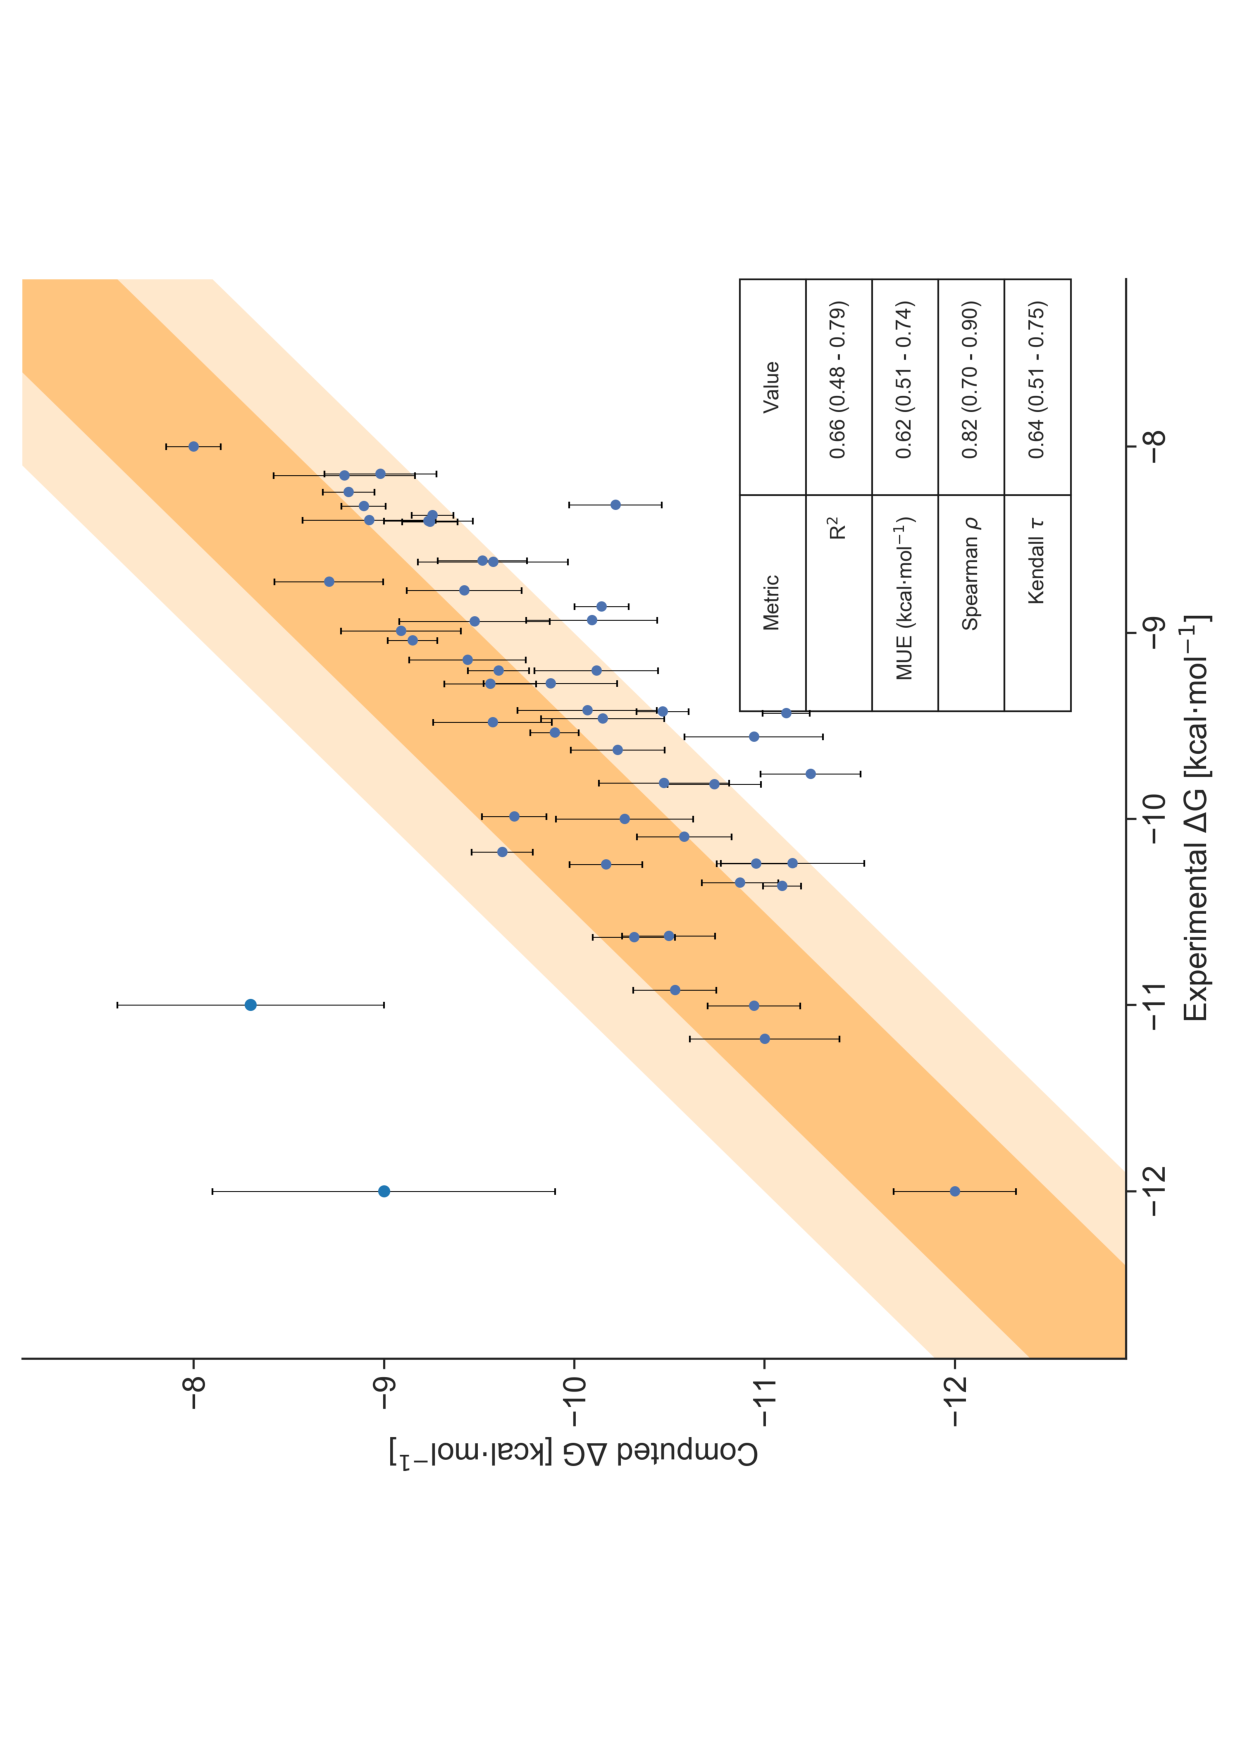
\includegraphics[width=0.95\columnwidth]{figures/fig6_types_of_networks/Figure.pdf}
    \caption{\textbf{Examples of perturbation networks} (\textbf{A}) Star shaped network with the crystal structure in the center. (\textbf{B}) Network with cycle closures (see more on this in Sec.~\ref{sec:are-they-good}). Arrows indicate the direction of the perturbation. Fully converged binding free energy calculations yield binding free energy changes which sum to zero around any closed cycle. However, in practice errors may not sum to zero around closed cycles, providing a way to look for potential sampling problems. Here in (B), green cycles indicate cycles with hypothetically good cycle closure, red those with poor cycle closure. The red arrow indicates a poorly converged simulation that would give rise to bad cycle closures. The diamond indicates the use of a crystallographic binding mode.}
    \label{fig:fig_types_of_networks}
\end{figure} 

In some cases, during the lead optimization stage, or for very large datasets that would benefit from rougher initial free energy ranking, or in cases where perturbations would be rather large, a star shaped network as seen in Fig.~\ref{fig:fig_types_of_networks} \textbf{A} is used. However, adding redundancy into the network means that a better error analysis can be carried out by looking at cycle closure errors as discussed in sec.~\ref{sec:are-they-good}, with an example given in Fig.~\ref{fig:fig_types_of_networks}\textbf{B}.


Methods from experimental design have been applied to the construction of the perturbation maps. Yang et al.~\cite{yang2020optimal} showed how to optimize the perturbation map by selecting a fixed number of calculations from the pairwise perturbations so that the resulting set of calculations minimize the total variance. Xu~\cite{xu2019optimal} showed how to optimize the perturbation map by allocating different amounts of simulation time to different pairwise perturbations so as to minimize the total variance, given the total simulation time of all the perturbation calculations. Both approaches lead to substantial reduction in the statistical error of the estimated free energies. 

{\color{blue}
\paragraph{Multistate methods}
When dealing with large datasets, methods that compute the binding free energies of multiple ligands simultaneously offer a compelling alternative to pairwise calculations. These approaches -- categorized as "multiple end state" or "multistate" free energy calculations -- sidestep ligand network construction entirely and provide all pairwise free energy differences directly with similar statistical uncertainties (i.e., cycle closure is given by definition). One potential disadvantage of multistate methods is, however, that the presence of multiple end states may complicate the energy landscape, thus requiring longer, inherently sequential simulations. Additionally, they are often more difficult to set up as the combination of multiple ligand topologies into a dual or hybrid topology raises extra challenges \cite{ries2022restraintmaker}.

A well-established method from this category is enveloping distribution sampling (EDS) \cite{christ2007enveloping}, which constructs a single reference state $R$ from the end-states, 
\begin{equation}\label{eq:eds}
H_R (\vec{q}) = - \beta s \ln{ \sum_{i=1}^N \left( e^{-\beta s (H_i(\vec{q})-E_i^R)}\right)},
\end{equation}
where $\vec{q}$ are the coordinates of the system, $\beta=(k_B T)^{-1}$ with $k_B$ being the Boltzmann constant and $T$ the absolute temperature, $N$ is the number of end-states, $s$ is the smoothing parameter and $E^R$ the energy offsets.
The computational efficiency of EDS is mainly due to the fact that interactions between unperturbed protein and solvent degrees of freedom have to be calculated only once regardless of $N$, provided a pairwise decomposable method like e.g. reaction field \cite{tironi1995generalized} is used for the long-range electrostatic interactions. Thus, the computational cost of adding more ligands grows approximately linearly rather than quadratically (in a fully connected perturbation graph) \cite{champion2023accelerating}.

To ensure sampling of all end-states in the EDS simulation, the reference-state parameters $s$ and $E^R$ must be optimized.
To simplify the calibration when $N >2$ and to improve the robustness of the methodology, multiple EDS reference-state potentials can be combined in a replica-exchange setup (termed RE-EDS) with different magnitudes of smoothing ($s$-parameter) \cite{sidler2016replica, sidler2017efficient, ries2022relative, champion2023accelerating}. 
RE-EDS simulations can be conducted using either a single or dual coordinate framework \cite{ries2022restraintmaker}. In the first case, all ligands must be restrained together (e.g. with distance restraints) to avoid diffusing out of the binding site. However, the number and definition of restraints should be chosen carefully as they can introduce bias in the simulations if not explicitly corrected. Single coordinate topologies (such as SCDT) can alleviate this issue as well as improve phase-space overlap \cite{champion2023accelerating} although their implementation in most MD engines usually requires custom routines.

RE-EDS implementations in the GROMOS \cite{champion2023accelerating} or OpenMM \cite{rieder2022leveraging} software packages include automated parameter calibration procedures (i.e., optimizing the distribution of replicas in smoothness-parameter space, optimizing the energy offsets). Previous work showed that 15-30 ligands can be treated in a RE-EDS simulations in practice without issues \cite{rieder2022leveraging, champion2023accelerating,champion2024multistate}.
However, sampling issues can occur for ligands that require insertion or deletion of many heavy atoms. In these cases, it is beneficial to split the set of ligands into smaller groups or include such a ligand via pairwise calculations.
}

\section{\tocred{How should I automate my calculations}}
\label{sec:automation}
\tocsectioncomment{Include e.g. automated selection of where to concentrate sampling time e.g. https://pubs.acs.org/doi/10.1021/acs.jctc.1c00703, automated selection of restraints for ABFE, link with discussion of available tools?}
\tocsectioncomment{@OpenFE team well placed to contribute. Discuss tools like alchemiscale? Discuss e.g. integration with REINVENT/ Maize for active learning?}

\section{\tocorange{Data analysis}}
\label{sec:data_ana}

\subsection{Uncertainty estimation}
\tocsubsectioncomment{@Agastya P Bhati/ Peter Coveney to cover uncertainty estimation for multiple simulations? Move cycle closure etc sections here.}
\label{subsec:uncertainty}

\paragraph{Cycle closure error}
Relative free energy calculations, which compute the change in free energy on making a change to a molecule (e.g. adding a functional group to a ligand) may provide an additional opportunity for error/consistency checking. Particularly, such calculations are often done to span a graph or tree of free energy calculations~\cite{xu2019optimal,wang2013modeling,liu2013lead}. In some cases the free energy change to go between molecules A and B can be obtained via multiple transformation pathways. This allows a type of consistency checking where we assess how much the free energy change for that transformation in practice differs from equivalence. 

Significant deviations of agreement from the same transformation by different routes  typically indicate insufficient configurational sampling along the lambda schedule of one or more of the transformations involved. This approach may be generalised to sets of connected transformations given the requirement that the sum of free energy changes along edges of a closed cycle should be zero. This analysis is called ``cycle closure''. In practice, such thermodynamic cycles do not actually sum to zero, and deviations become increasingly large as the size of the cycle increases owing to propagation of error. Though no firm guidelines have emerged, it may be judicious to perform additional configurational sampling along edges of a network that are involved in cycles closing poorly. This may be done by extending the duration of simulations, or by averaging free energy changes over multiple repeats. The latter approach may yield more reproducible free energy changes, but at the expense of a stronger bias on the estimated free energies due to repeated use of the same input coordinates.

A scheme to reduce cycle closure errors is used in FEP+ whereby calculated free energy changes along the nodes of the network are re-sampled assuming estimates of the calculated free energy change along a node may be obtained from a Gaussian distribution centered on the estimated free energy change and with a standard deviation equal to the estimated standard deviation of the free energy change. The procedure then uses a maximum likelihood method to find new sets of free energy changes that minimize cycle closure errors~\cite{wang2013modeling}. An alternative approach computes the free energy change between a target and reference compound as a weighted average over all unique paths in the network, with the weights derived from the propagated uncertainties of each node~\cite{mey2016blinded}. Approaches as illustrated by Yang et al. for perturbation map design can also be used to compute relative free energies between target and reference compounds~\cite{yang2020optimal}.

\subsection{Best practices for reporting data }
\label{sec:plot_data}
\tocsubsectioncomment{@OpenFE team/ @Jenke Scheen/ Volunteers to expand on utility/ limitations of common metrics. Also see @Michael Gilson's GitHub issue.}
Following best practices for data generation and their analysis does not mean that data is reported in the optimal way. As a practitioner of alchemical free energy simulations you also should use best practices for reporting and plotting your results. We encourage the following standard set of analyses and ways to represent data. 
\paragraph{Statistics to include in reporting data}
As with any modelling technique, misuse of statistical analysis can skew the perception of how well models perform in free energy predictions. First, error estimates should always be included on your predictions in whatever form you present your data (scatterplots, barplots, etc; see next paragraph). We recommend performing triplicates of your predictions at minimum, with starting points that are expected to be uncorrelated, to ensure some measure of reliability in your data. This replication may seem excessive, but uncertainty estimates often underestimate the true statistical uncertainty. Where performing multiple replicas of the simulation is not possible, an error estimate from e.g. MBAR can be used, though bearing in mind this is likely an underestimated error. 

As alchemical free energy methods are used in drug discovery to quantify and rationalise structure activity relationships (SAR), the models ability to (a) correlate well with experiment and (b) rank-order the molecules by affinity, should both be computed. Conventionally, this means including an R\textsuperscript{2} (or Pearson's R), where $R=+1$ means high correlation, $R=0$ means no correlation, and $R=-1$ means high anti-correlation) and a Kendall \texttau{} (with perfect ranking agreement when \texttau=1 and perfect disagreement when \texttau=-1) metric in your results. Additionally, practitioners may choose to include a Spearman \textrho{} as well. Brown et al.~\cite{brown2009healthy} have provided a useful analysis in terms of upper bounds of expected possible correlations between experiment and computation with a given potency range for the compounds. For example, for potency ranges of 2 log units it would be impossible to get a higher correlation in R than 0.8 because of experimental uncertainties~\cite{brown2009healthy}. What often is neglected to include is an error analysis on correlation statistics that arise from the errors of both experimental and computed data. One way to include such error analysis for correlation metrics is using bootstrapping on the datasets. The D3R community challenges follows best practices on their data evaluation with readily available python scripts online~\cite{2018drugdata}, based on work by Pat Walters~\cite{walters2013what}. Other analysis software also provide similar functionality for bootstrapping datasets~\cite{antonia2019michellab}. 

Mean unsigned error (MUE, also called mean absolute error/MAE) is another key statistic to include in your results. Even though some models' near-perfect correlation and ranking statistics might suggest excellent accuracy, MUE values can still have errors of multiple kcal/mol, providing important additional insight into performance. Furthermore, MUE allows for unbiased comparisons between predictive models as it is less sensitive to dataset size. Other metrics such as Gaussian Random Affinity Model (GRAM)~\cite{cui2020gram}, Predictive Interval (PI) and Relative Absolute Error (RAE), attempt to correct for the inherent potency range of a dataset, which can aid in comparing success between different targets. We recommend further reading on evaluation of computational models~\cite{jain2008recommendations, walters2013what, brown2009healthy, walterthoughts}.

Reporting the results of relative free energy calculations requires care. As shown in Fig.~\ref{fig:fig_types_of_networks}, relative free energies can be performed arbitrarily as a forward or a reverse process, and thus relative free energies may be reported as either positively or negatively valued. The consequence of the two possible signs for relative free energies is that correlation statistics (such as Pearson's R and Kendall \texttau{}) can be skewed depending on which sign is analysed. The issue of this inconsistency can be circumvented by either plotting all datapoints within a consistent quadrant~\cite{perez-benito2019predicting}, or by avoiding the use of correlation statistics for assessment of relative free energy calculations and instead measuring accuracy using RMSE and MUE, which are unaffected by choice of sign.


\paragraph{Presenting your data}
As essentially all alchemical free energy prediction schemes are regression problems, the preferred type of plot is a scatter plot (see Fig.~\ref{fig:scatterplot_analysis}). Most alchemical free energy projects will look at 10-50 ligands. Any study with \textless10 ligands is more suitable for bar plots (with inclusion of error bars), and is unlikely to provide meaningful statistics. Any study with \textgreater50 ligands typically contains multiple protein targets to which alchemical free energies may perform better on some targets than others. Because of this, it is bad practice to place multiple datasets on the same plot as this can suggest high model accuracy even though the individual models perform less well~\cite{walterthoughts}.

\begin{figure}
  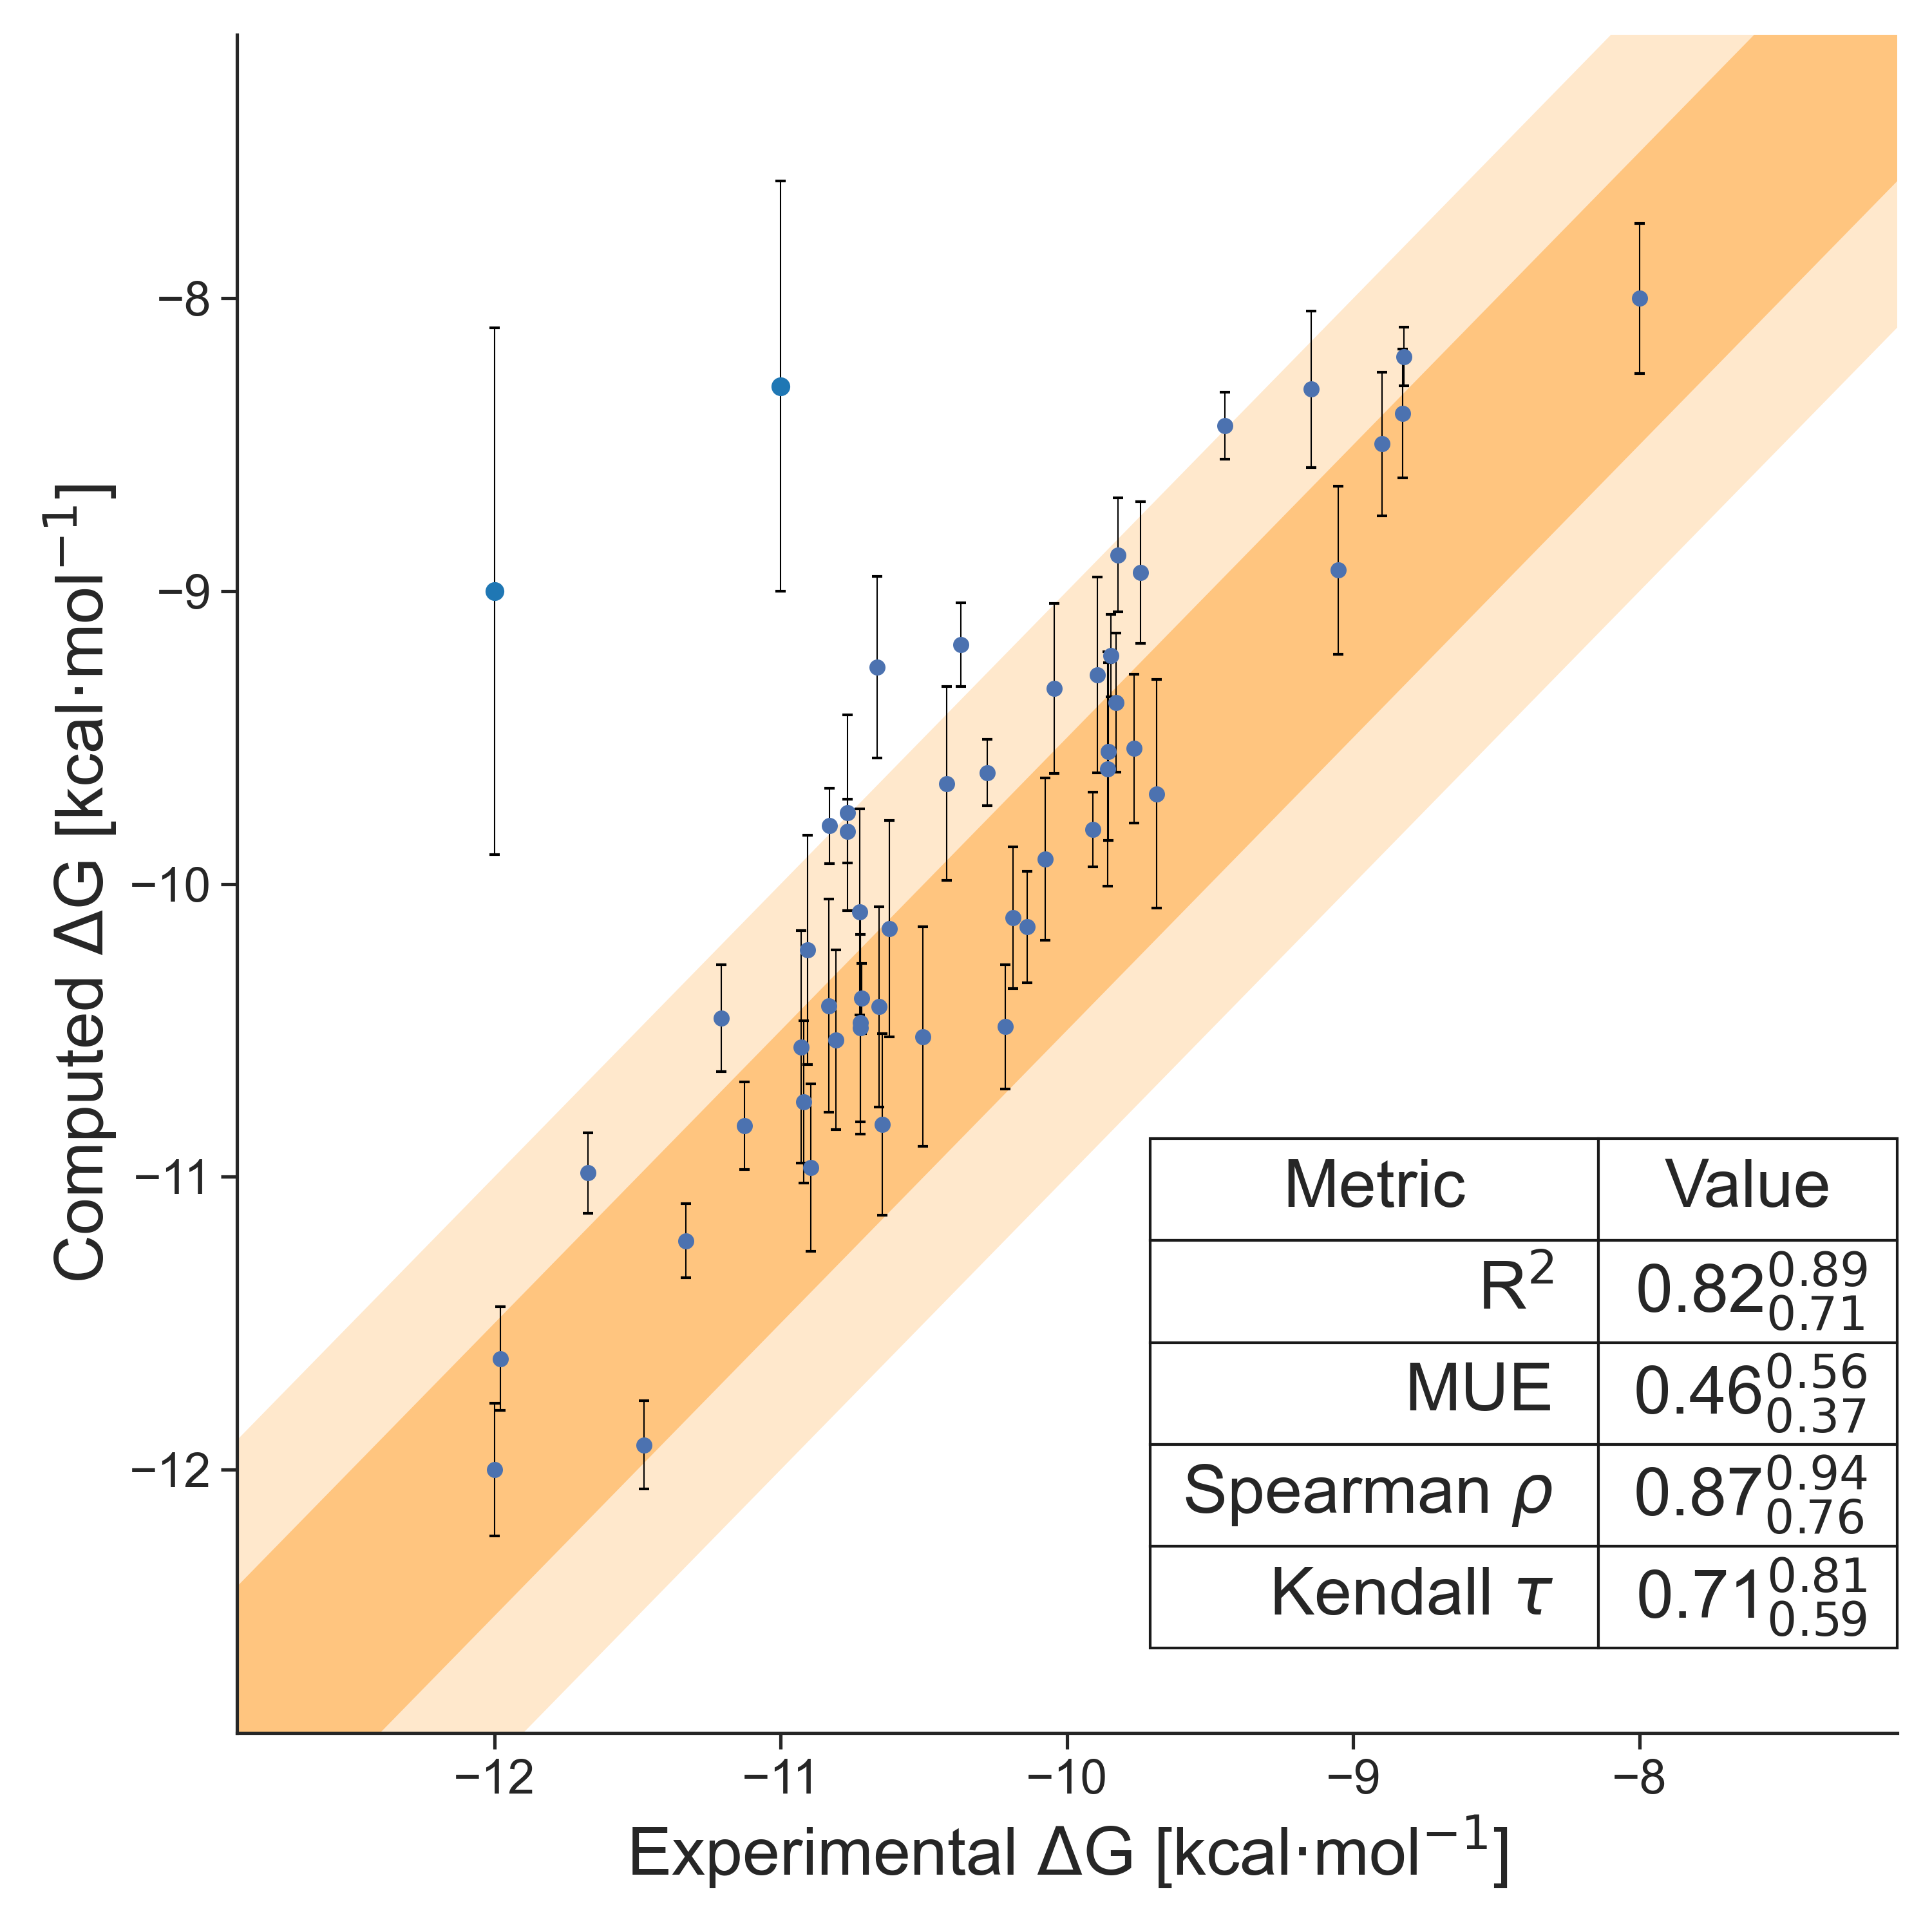
\includegraphics[width=0.95\linewidth]{figures/fig13_analysis_practices/Figure.png}
  \caption{\textbf{An example of recommended practices for graphing alchemical free energy predictions.} This figure shows the relation between predicted and experimentally-determined Gibbs free energy in kcal/mol with standard errors as error bars. The dark and light-orange regions depict the 1- and 2-kcal/mol confidence bounds. Statistical metrics for the data are reported, with 95\% confidence intervals determined by bootstrapping analysis. Extra care should be taken when investigating potential outliers further.}
   \label{fig:scatterplot_analysis}
\end{figure}

As we are interested mainly in the linear relationship between the alchemical free energy predictions and the experimentally-determined affinity values, plots should be depicted with the same range on both axes (i.e. $x=y$) with a 1:1 aspect ratio, with units for both experiment and simulation converted to be the same. If this skews the plot to a point where it is difficult to read of information, using the same dimensions, such that e.g. 1 cm is 1 kcal/mol is acceptable. Furthermore, bounds should be depicted for the 1- and 2-kcal/mol confidence regions. These regions can serve as tools to communicate your model performance: any predictions inside the 1 kcal/mol region can be seen as highly reliable, any predictions inside the 2 kcal/mol region should be seen as somewhat reliable, and any predictions outside the confidence regions should be expected to be unreliable and handled as outliers. In a drug discovery context, this type of data depiction may suggest the reliability of alchemical FE predictions in the project, and can give an idea of how trustworthy predictions can be for synthesis ideas. It is also recommended to included experimental error bars in all plots.

An example of a best practice scatter comparison between computed and experimental values is shown in Fig.~\ref{fig:scatterplot_analysis}, highlighting outliers, error bars and confidence intervals. The data for this plot is artificially generated for illustration purposes.


\section{\tocred{Unsettled Practices and Current Limitations}}
\tocsectioncomment{@Everyone to contribute to section on unsettled practices/ current limitiations, as suggested by John Chodera.}
\label{sec:unsettled}

\subsection{Unsettled practices}
\tocsubsubsectioncomment{Include discussion of active learning/ fast ABFE for virtual screening?}

\subsection{Current limitations}

\section{\tocred{Conclusion}}
\tocsectioncomment{@Volunteer to add.}
\label{sec:conclusion}

%%%%%%%%%%%%%%%%%%%%%%%%%%%
%  Benchmark information  %
%%%%%%%%%%%%%%%%%%%%%%%%%%%
\section{\tocorange{Alchemical free energy datasets: an overview}}
\tocsectioncomment{@Volunteers to update this section}
\label{sec:benchmark}
The following contains a non-exhaustive summary of alchemical free energy datasets that can serve as a starting point to review approaches or test new implementations. The field is moving towards a more standardised way of generating protein-ligand benchmark datasets and the progress of these efforts can be tracked here: \url{https://github.com/openforcefield/FE-Benchmarks-Best-Practices}. Currently lacking an exhaustive set of benchmark datasets, the review by Williams-Noonan et al.~\cite{williams-noonan2018free} contains an overview of recently published alchemical free energy studies. For comparison of FEP+ and Gromacs (using the AMBER99SB-ILDN and GAFF2 force field), cf. the recently published study by Pérez-Benito et al.~\cite{perez-benito2019predicting}.
An overview of further suggested benchmark sets can be found in the review by Mobley and Gilson~\cite{mobley2017predicting} or on \url{alchemistry.org}~\cite{alchemistry}. These include cyclodextrins, the Cytochrome C peroxidase (CCP) protein model binding site, thrombin and bromodomains as well as solvation benchmark sets~\cite{paliwal2011benchmark}. Please refer to table~\ref{tab:benchmarks}, for a small overview of datasets, what forcefields they used, and what the original study was it came from. 

\begin{table}
\caption{Selection of example datasets}
\begin{tabular}{cccc}
\textbf{Publication} & \textbf{Targets} & \textbf{Ligands} & \textbf{Force Field} \\
\hline
\multicolumn{4}{|c|}{D3R Grand Challenges~\cite{D3R}} \\
\hline
GC3~\cite{gaieb2019d3r} & 6 & 266 & various \\
GC2~\cite{gaieb2018d3r} & 1 & 102 & various \\
GC2015~\cite{gathiaka2016d3r} & 2 & 215 & various \\
\hline
\multicolumn{4}{|c|}{SAMPL Challenges~\cite{SAMPL}} \\
\hline
SAMPL6~\cite{rizzi2018overview} & 3 & 21 & various \\
SAMPL5~\cite{yin2017overview} & 3 & 22 & various \\
SAMPL4~\cite{muddana2014sampl4} & 2 & 23 & various \\
\hline
\multicolumn{4}{|c|}{Schrödinger Datasets} \\
\hline
FEP+ Dataset~\cite{wang2015accurate} & 8 & 199 & OPLS2.1 \\
FEP+ Dataset~\cite{harder2016opls3} & 8 & 199 & OPLS3 \\
FEP+ Dataset~\cite{roos2019opls3e} & 8 & 199 & OPLS3e \\
FEP+ Dataset~\cite{song2019using} & 8 & 199 & GAFF 1.8 \\
FEP+ Dataset~\cite{gapsys2020large} & 8 & 199 & various \\
FEP+ Dataset~\cite{kuhn2020assessment} & 8 & 199 & GAFF2.1 \\
Fragments ~\cite{steinbrecher2015accurate} & 8 & 96 & OPLS2.1 \\
Scaffold Hopping~\cite{wang2017accurate} & 6 & 21 & OPLS3 \\
Scaffold Hopping~\cite{kuhn2020assessment} & 6 & 21 & GAFF2.1 \\
Macrocycles~\cite{yu2017accurate} & 7 & 33 & OPLS3 \\
\hline
\multicolumn{4}{|c|}{Further Suggested Datasets} \\
\hline
Cucurbit[7]uril (CB7)~\cite{mobley2017predicting} & 1 & 15 & NA \\
Deep cavity cavitand~\cite{mobley2017predicting} & 2 & 19 & NA \\
T4 Lysozyme~\cite{mobley2017predicting} & 2 & 20 & NA \\
Merck set~\cite{MCompChem2019Sep} & 5 & 169 & OPSL3 \\

\hline
\label{tab:benchmarks}
\end{tabular}
\end{table}

\section{\tocorange{Checklist}}
\tocsectioncomment{@Volunteer to update checklist once manuscript is nearing completion.}
\label{sec:checklist}
\begin{Checklists*}
\begin{checklist}{ Know what you want to simulate}
    \textbf{Initial questions you should ask before you set up an alchemical free energy calculation using molecular dynamics simulations}
\begin{itemize}
    \item Do I understand the biology, chemistry and physics of my system?
    \item Have I properly prepared my protein and ligand systems?
    \item Does my system contain any structures that require custom parameters?
    \item What simulation protocol will provide the most evidence to verify my hypothesis?
    \item Are the projected computational expense and runtime realistic for my scientific goals?
    \item Will my protocol be reproducible? 
    \item Will my statistics be reliable? If not, would more replicates solve the problem? 
    \item Can I open-source my data?
\end{itemize}
\end{checklist}

\begin{checklist}{Preparing your simulations}
\textbf{Steps to getting started setting up your alchemical free energy calculation}
\begin{itemize}
    \item Make sure you know why you have picked your (combination of) force field(s)
    \item Energy minimize your system
    \item Equilibrate your system properly with your choice of thermodynamic ensemble
    \item Check the stability of your system and whether it behaves the way you believe it should
\end{itemize}
\end{checklist}

\begin{checklist}{Running absolute simulations}
        \textbf{Steps to running your absolute alchemical free energy calculations}
\begin{itemize}
 \item Check your ligands have the same, biologically correct binding pose
        \item Make sure your \textlambda-scheduling is  appropriate
        \item Check if your ligands are discharging and decoupling correctly
        \item Set up your restraints correctly
        \item Make sure you subsample the data in your free energy estimation protocol
        \item Apply the appropriate correction terms
\end{itemize}
\end{checklist}

\begin{checklist}{Running relative simulations}
        \textbf{Steps to running your relative alchemical free energy calculations}
\begin{itemize}
   \item Check your ligands  have the same, biologically correct binding pose
        \item Make sure your $\lambda$-scheduling is set correctly
        \item Make sure your molecular transformations are realistic (1-5 heavy atoms for reliable computations)
        \item Generate a perturbation network by your method of choice; check whether you have enough cycle closures to check consistency in the results
        \item Check whether dummy atoms were assigned correctly
        \item Consider subsampling the data in your free energy estimation protocol
        \item Apply the 
        appropriate correction terms
\end{itemize}
\end{checklist}
\end{Checklists*}

%Analyis checklist
\begin{Checklists*}
\begin{checklist}{How do I know which simulations are unreliable?}
    \textbf{Situations suggesting your relative alchemical free energy calculations have not run properly (assuming absence of experimental affinities)}
        \begin{itemize}
                \item Standard error (\textsigma) should not be \textgreater1 kcal·mol$^{-1}$ 
    \item Simulated systems have not converged - trajectories should be manually checked for consistency; other methods such as generating RMSD plots are also recommended
    \newline\newline\textit{Relative:}
    \item If you observe hysteresis in perturbations and incorrect cycle closures
    \item Energy differences \textgreater$\sim$15 kcal$\cdot$mol$^{-1}$  are likely unreliable
    \newline\newline\textit{Absolute:}
    \item Energies \textless$\sim$-15 kcal$\cdot$mol$^{-1}$  are likely unreliable
    \item The ligand has not sampled most of the intended region after the decoupling step
    \item The ligand is drifting out of the intended region after the decoupling step
        \end{itemize}
\end{checklist}

\begin{checklist}{Why are they not reliable?}
    \textbf{Suggestions for finding out why your alchemical free energy calculations may not be reliable}
\begin{itemize}
    \item Check again whether dummy atoms were assigned correctly
    \item Inspect the trajectories across the $\lambda$-schedule (particularly the endpoints) for problems described in the text
    \item Inspect the overlap matrices for lack of overlap
\end{itemize}
\end{checklist}

\begin{checklist}{Data Analysis}
    \textbf{Steps to analyzing your output data correctly}
\begin{itemize}
    \item Make sure you have run enough replicates to ensure statistical reliability (\textgreater3)
    \item Compute both correlation and ranking coefficients and ranking statistics (e.g. r, \textrho, MUE and \texttau)
    \item Include error bars in all your visual analyses
\end{itemize}
\end{checklist}
\end{Checklists*}
\clearpage


\section*{Author Contributions}
%%%%%%%%%%%%%%%%
% This section mustt describe the actual contributions of
% author. Since this is an electronic-only journal, there is
% no length limit when you describe the authors' contributions,
% so we recommend describing what they actually did rather than
% simply categorizing them in a small number of
% predefined roles as might be done in other journals.
%
% See the policies ``Policies on Authorship'' section of https://livecoms.github.io
% for more information on deciding on authorship and author order.
%%%%%%%%%%%%%%%%
\textbf{ASJSM}: Coordinated the document, contributed to most sections, and co-designed Figs.~\ref{fig:fig_binding_thermodynamic_cycle},~\ref{fig:fig_topology},~\ref{fig:fig_mcss},~\ref{fig:fig_types_of_networks},~\ref{fig:fig_absolute_thermodynamic_cycle},~\ref{fig:scatterplot_analysis}, and created Figs.~\ref{fig:fig_what_is_lambda},~\ref{fig:fig_what_is_alchemy},~\ref{fig:overlap},~\ref{fig:pmf} and replotted~\ref{fig:automatic-equilibration-detection} and~\ref{fig:fig_types_of_networks}.\\
\textbf{BA}: Helped write the uncertainty estimation, stopping conditions, and output analysis sections and created figure ~\ref{fig:convergence_forward_reverse}.\\
\textbf{HBM} Contributed to Sec.~\ref{sec:plot_data} and Fig.~ \ref{fig:scatterplot_analysis} and helped edit the paper.\\
\textbf{JDC}: Wrote Sec.~\ref{sec:decorrelating-samples} and~\ref{sec:automatic-equilibration-detection} discussed structure and design of the whole document, suggested Figs.~\ref{fig:fig_what_is_alchemy} and~\ref{fig:fig_sampling_scheme}. \\
\textbf{DFH} Contributed to Sec.~\ref{sec:software} and helped edit the paper. \\
\textbf{MK}: Contributed to Sec.~\ref{sec:data_analysis}, provided the data for figure~\ref{fig:overlap}, compiled the dataset for Sec.~\ref{sec:benchmark} and helped edit the paper.\\
\textbf{JM}: Contributed to Sec.~\ref{subsec:reproducible},~\ref{sec:prerequisites},~\ref{sec:important_path},~\ref{subsec:estimators},~\ref{subsec:uncertainty}, and~\ref{sec:conclusion}\\
\textbf{DLM}: Contributed to the outline, drafted some of the sections, gave ideas on figures, and helped edit the paper.\\
\textbf{LNN}: Helped write the simulation length, stopping conditions, and information saving section. Edited and reviewed alchemical path section.\\
\textbf{SP} Wrote Sec.~\ref{sec:software}. \\
\textbf{AR}: Created figure~\ref{fig:freeenergytrajectories}, contributed to sections~\ref{sec:theory} and~\ref{sec:simulation_protocol_choice}, and helped edit the paper.\\
\textbf{JS}: Created Figs.~ \ref{fig:fig_what_is_alchemy},~\ref{fig:fig_binding_thermodynamic_cycle},~\ref{fig:fig_topology},~\ref{fig:fig_mcss},~\ref{fig:fig_absolute_thermodynamic_cycle},~\ref{fig:scatterplot_analysis}, and an initial draft of~\ref{fig:fig_types_of_networks}. Wrote Sec.~\ref{sec:plot_data}, the checklist Sec.~\ref{sec:checklist}, and contributed to general formatting discussions and editing.\\
\textbf{MRS}: Helped create figure~\ref{fig:fig_what_is_lambda}, wrote Sec.~\ref{sec:important_path} describing choices for alchemical pathways and parts of~\ref{sec:data_analysis} on the analysis for free energy calculations. Reviewed and edited text throughout.\\
\textbf{GT}: Contributed to Sec.~\ref{sec:intro} and~\ref{sec:problem_suitable}, and helped edit the paper.\\
\textbf{HX}: Contributed Sec.~\ref{subsec:accuracy}, to Sec.~\ref{sec:relative-fe-protocol}, and to Sec.~\ref{sec:are-they-good}.
% We suggest you preserve this comment:
For a more detailed description of author contributions,
see the GitHub issue tracking and changelog at \githubrepository.

\section*{Other Contributions}
%%%%%%%%%%%%%%%
% You should include all people who have filed issues that were
% accepted into the paper, or that upon discussion altered what was in the paper.
% Multiple significant contributions might mean that the contributor
% should be moved to authorship at the discretion of the a
%
% See the policies ``Policies on Authorship'' section of https://livecoms.github.io for
% more information on deciding on authorship and author order.
%%%%%%%%%%%%%%%
Julia E. Rice participated in the original discussion of the document at the Best Practices in Molecular Simulation Workshop Hosted by at NIST, Gaithersburg, MD, August 24th-25th, 2017.
Marieke Schor proofread the manuscript. 

% We suggest you preserve this comment:
For a more detailed description of contributions from the community and others, 
see the GitHub issue tracking and changelog at \githubrepository.


\section*{Potentially Conflicting Interests}
%%%%%%%
%Declare any potentially competing interests, financial or otherwise
%%%%%%%
JM is a current member of the Scientific Advisory Board of Cresset. 
MK is employed by Cresset who commercially distribute a software for performing alchemical free energy calculations. MRS is a Open Science Fellow and consultant for Silicon Therapeutics.
JDC is a current member of the Scientific Advisory Board of OpenEye Scientific Software and a consultant to Foresite Laboratories.
\section*{Funding Information}
%%%%%%%
% Authors should acknowledge funding sources here. Reference specific grants.
%%%%%%%
ASJSM and JM acknowledge funding through an EPSRC flagship software grant: EP/P022138/1
MK and JM acknowledge funding through Innovate UK by KTP partnership 011120.
AR acknowledges partial support from the Tri-Institutional Program in Computational Biology and Medicine and the Sloan Kettering Institute.
HEBM acknowledges support from a Molecular Sciences Software Institute Investment Fellowship and Relay Therapeutics.
DLM acknowledges support from the National Institutes of Health (R01GM108889, R01GM124270, and R01GM132386), and the National Science Foundation (CHE 1352608).
JDC acknowledges support from the National Institutes of Health (NIH P30 CA008748, NIH R01 GM121505, R01 GM132386).
A complete funding history for the Chodera lab can be found at \url{http://choderalab.org/funding}.
The content is solely the responsibility of the authors and does not necessarily represent the official views of the National Institutes of Health.

\section*{Author Information}
\makeorcid
\bibliography{alchemical,manual}

%%%%%%%%%%%%%%%%%%%%%%%%%%%%%%%%%%%%%%%%%%%%%%%%%%%%%%%%%%%%
%%% APPENDICES
%%%%%%%%%%%%%%%%%%%%%%%%%%%%%%%%%%%%%%%%%%%%%%%%%%%%%%%%%%%%

%\appendix


\end{document}
